\section{Basic principles} \label{sec:basic_filter}
A digital filter is characterised as an LTI system as previously defined by equation \eqref{eq:LTI_diff_equation_finite}. As described, the system is completely characterised by its corresponding impulse response $h[n]$. In terms of the filter as an LTI the output $y[n]$ is the part of the signal that passes through the filter. \\
$y[n]$ has previously been defined by \eqref{def:convolution} as the convolution sum of the input signal $x[n]$ and the impulse response of the system:
\begin{align*}
y[n] = x[n]*h[n] = \sum_{k=-\infty}^{\infty} x[k]h[n-k].
\end{align*}

The frequency response of the system is given by the Fourier transform of the impulse response as
\begin{align} \label{eq:freq_res}
H(\omega) = \sum_{k=-\infty}^{\infty} h[k] \text{e}^{-j\omega k}.
\end{align}

$H(\omega)$ can be expressed as the \textit{amplitude response} $|H(\omega)|$ and \textit{phase response} $\text{e}^{j\measuredangle H(\omega)}$ of the filter:
\begin{align*}
H(\omega) = |H(\omega)| \text{e}^{j\measuredangle H(\omega)}.
\end{align*}

The amplitude and phase response are both real valued and $2\pi$-periodic. If $H(\omega)$ is real it is said to have \textit{zero phase}, which is equivalent to the phase response only taking values that are integer multiples of $\pi$, resulting in a straight phase with zero slope \cite{page 227, FSP}. Furthermore, if $H(\omega)$ can be written on the form
\begin{align} \label{eq:lin_pha}
H(\omega) = A(\omega) \text{e}^{j(-\alpha\omega + \beta)},
\end{align}

where $\alpha$ and $\beta$ are constants and $A(\omega)$ is real, the filter is said to have \textit{generalized linear phase}. This is due to the phase response consisting of constant terms added to the linear function making a straight line with slope $\alpha$ except from the discontinuities resulting from jumps of $2\pi$ caused by the $2\pi$-periodicity. \\
A generalized linear phase response is characterized by a constant \textit{group delay} $\tau(\omega)$:
\begin{align*}
\tau(\omega) = \text{grd}[H(\omega)] = -\frac{d}{d\omega} \left\{ \measuredangle H(\omega) \right\} = \alpha.
\end{align*}

The frequency response with general linear phase as described in \ref{eq:lin_pha} may further be written as
\begin{align*}
H(\omega) = A(\omega) \text{e}^{j(-\alpha\omega + \beta)} = A(\omega) \cos(-\alpha\omega + \beta) + j A(\omega) \sin(-\alpha\omega + \beta),
\end{align*}

which is equivalent to
\begin{align*}
H(\omega) = \sum_{n=-\infty}^\infty h[n] \text{e}^{-j \omega n} = \sum_{n=-\infty}^\infty h[n] \cos(\omega n) - j \sum_{n=-\infty}^\infty h[n] \sin(\omega n),
\end{align*}

where it is assumed that $h[n]$ is real. The tangent of the phase angle of $H(\omega)$ can be expressed as
\begin{align*}
\tan(-\alpha\omega + \beta) = \dfrac{\sin(-\alpha\omega + \beta)}{\cos(-\alpha\omega + \beta)} = \dfrac{- \sum_{n=-\infty}^\infty h[n] \sin(\omega n)}{\sum_{n=-\infty}^\infty h[n] \cos(\omega n)}.
\end{align*}

Cross multiplying leads to the following condition for the system to have constant group delay \cite{page 341, DTSP}:
\begin{align}\label{eq:cons_gro}
\sum_{n=-\infty}^{\infty}h[n]\sin\left(\omega \left(n-\alpha \right) + \beta \right) = 0.
\end{align}

for all $\omega$. This is a necessary condition but not a sufficient condition, however. The phase response is an expression of how each of the signal components are delayed through the system, where linear phase indicates an equal delay for all components of the signal. The generalized linear phase is further described in section \ref{sec:FIR_IIR}.

\subsection{Ideal filters} \label{sec:ideal_filt}
When designing filters it is ideal to have constant amplitude and zero phase corresponding to the frequency response. For an ideal selective frequency filter the amplitude response will be constant unity for the frequencies that are wanted to pass the filter and zero for all other frequencies. These bands are referred to as \textit{bandpass} and \textit{bandstop}. An example is an ideal lowpass filter with frequency response 
\begin{align} \label{eq:low}
H_{lp}(\omega) =
\left\{ \begin{matrix}
1, &\ \left| \omega \right|< \omega_c \\
0, &\ \omega_c < \left| \omega \right| \leq \pi
\end{matrix}\right.,
\end{align}
    
where $H_{lp}(\omega)$ is $2\pi$-periodic and $\omega_c$ is referred to as the \textit{cut-off frequency}. The lowpass filter selects the frequencies lower than the cut-off frequency and rejects the higher frequency components of the input signal. By \eqref{eq:low} it is seen that the lowpass filter is real valued, and hence it has zero phase as expected. \\
The corresponding impulse response is determined by the inverse Fourier transform on the passband interval
\begin{align} \label{eq:low_im}
h_{lp}[n] = \frac{1}{2\pi} \int_{-\pi}^{\pi} H_{lp}(\omega) \text{e}^{j\omega n} d\omega = \dfrac{1}{2\pi}\int_{-\omega_c}^{\omega_c}\text{e}^{j\omega n} d\omega = \dfrac{1}{2\pi j n}\left[\text{e}^{j\omega n} \right]_{-\omega_c}^{\omega_c} = \dfrac{\sin(\omega_c n)}{\pi n}
\end{align}

for $-\infty < n < \infty$. Note that the second equality is true since the integral is zero outside the interval $[-\omega_c, \omega_c]$ according to \eqref{eq:low}. \eqref{eq:low_im} only holds for values $n \neq 0$, and thus $h_{lp}[0]$ must be defined separately. It follows that
\begin{align*}
h_{lp}[0] = \dfrac{1}{2\pi} \int_{-\pi}^\pi H_{lp}(\omega) \text{e}^{-j \omega \cdot 0} d\omega = \dfrac{1}{2\pi} \int_{-\omega_c}^{\omega_c} 1 \ d\omega = \dfrac{1}{2\pi} \left[ \omega \right]_{\omega = -\omega_c}^{\omega_c} = \dfrac{\omega_c}{\pi}
\end{align*}

since $H_{lp}(\omega) = 1$ for $|\omega| < \omega_c$ and $0$ otherwise.
\\ \\
By \eqref{eq:low_im} the impulse response is non-zero for all $n<0$, and thus the filter is non-causal according to definition \ref{def:causal_system}.
The amplitude and impulse responses of the ideal lowpass filter are illustrated on figure \ref{fig:ideal_low}.

\begin{figure}[H]
\begin{subfigure}[b]{0.50\textwidth}
        \centering
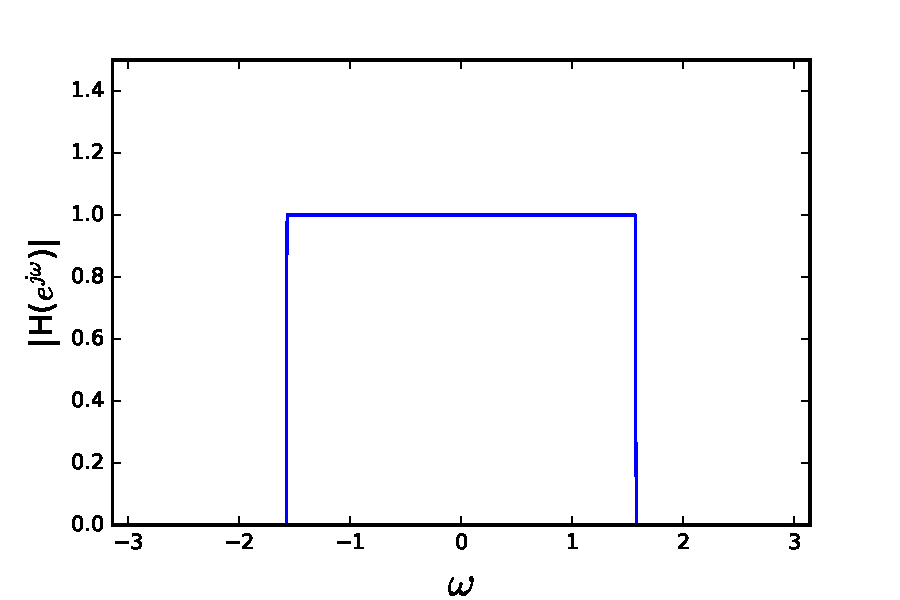
\includegraphics[scale=0.45]{figures/filter_teori/ideal_low2.pdf}
\caption{}
\end{subfigure}
\begin{subfigure}[b]{0.50\textwidth}
        \centering  
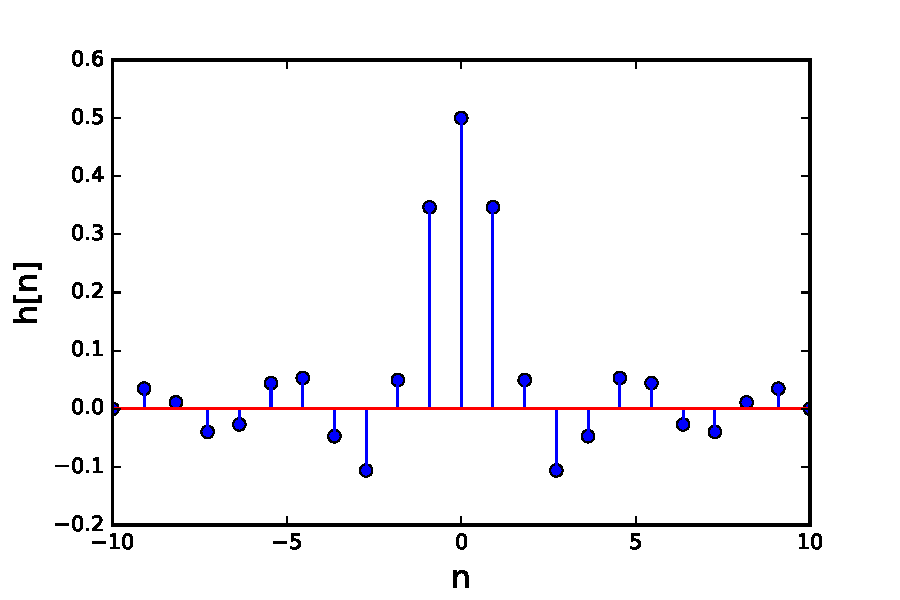
\includegraphics[scale=0.45]{figures/filter_teori/ideal_low1.pdf}
\caption{}
 \end{subfigure}
\caption{\textbf{(a)} Amplitude response of ideal lowpass filter centered around $\alpha=0$ with $\omega_c = \frac{\pi}{2}$ and \textbf{(b)} the corresponding impulse response.}
\label{fig:ideal_low}
\end{figure}

Ideal highpass and bandpass filters can be defined analogues to a low pass filter as illustrated on figure \ref{fig:ideal}.

\begin{figure}[H]
\begin{subfigure}[b]{0.50\textwidth}
        \centering
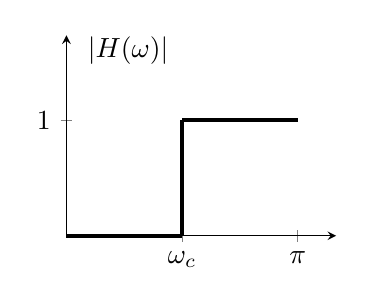
\begin{tikzpicture}[scale=1]
\begin{axis}[
clip=false,
scale=0.5,
unit vector ratio*=1 1 1,
axis lines = middle,
xtick={1.5,3},
xticklabels={$\omega_c$,$\pi$},
ytick={1.5},
yticklabels={$1$},
xmin=0,
xmax=3.5,
ymin=0,
ymax=2.6]
\node at (axis cs:0.8,2.4) {$|H(\omega)|$};
\draw[line width=0.5mm](axis cs:0,0)--(axis cs:1.5,0);
\draw[line width=0.5mm](axis cs:1.5,1.5)--(axis cs:3,1.5);
\draw[line width=0.5mm](axis cs:1.5,1.5)--(axis cs:1.5,0);
\end{axis}
\end{tikzpicture}

\caption{}
    \end{subfigure}
 \begin{subfigure}[b]{0.50\textwidth}
        \centering  
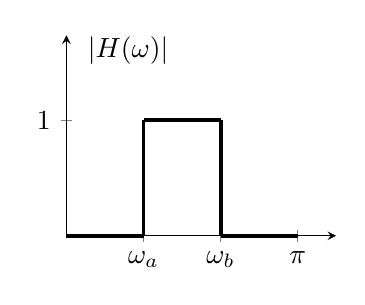
\begin{tikzpicture}[scale=1]
\begin{axis}[
clip=false,
scale=0.5,
unit vector ratio*=1 1 1,
axis lines = middle,
xtick={1,2,3},
xticklabels={$\omega_a$,$\omega_b$,$\pi$},
ytick={1.5},
yticklabels={$1$},
xmin=0,
xmax=3.5,
ymin=0,
ymax=2.6]
\node at (axis cs:0.8,2.4) {$|H(\omega)|$};
\draw[line width=0.5mm](axis cs:1,1.5)--(axis cs:1,0);
\draw[line width=0.5mm](axis cs:1,1.5)--(axis cs:2,1.5);
\draw[line width=0.5mm](axis cs:2,1.5)--(axis cs:2,0);
\draw[line width=0.5mm](axis cs:1,0)--(axis cs:0,0);
\draw[line width=0.5mm](axis cs:2,0)--(axis cs:3,0);
\end{axis}
\end{tikzpicture}
\caption{}
    \end{subfigure}
\caption{Amplitude responses of ideal \textbf{(a)} highpass filter and \textbf{(b)} bandpass filter.}
\label{fig:ideal}
\end{figure}
An ideal filter with zero phase is non-causal and as stated in section \ref{sec:LTI} a non-causal LTI system is not realizable. Thus an approximation of an ideal filter needs to be computed by a causal system with generalized linear phase.

\section{FIR and IIR filters} \label{sec:FIR_IIR}
Two classes of filters are essential to identify. For all ideal filters discussed in the previous section the impulse response is defined for $-\infty < n < \infty$. Such a filter is specified as an \textit{infinite impulse response (IIR)} filter which is not further explained in this section. In the case of the impulse response being zero outside a finite interval the filter is referred to as a \textit{finite impulse response (FIR)} filter which is shown to have generalized linear phase.

\subsection{FIR filters}
As described previously, causal systems with generalized linear phase is a possible approximation of the ideal filter. This is to be guaranteed by using specific types of FIR filters. A causal system with generalized linear phase has to fulfil the following relation for all $\omega$ as described in section \ref{sec:basic_filter}:
\begin{align*}
\sum_{n=0}^{\infty}h[n]\sin\left(\omega \left(n-\alpha \right) + \beta \right) = 0.
\end{align*}
The point of symmetry for an FIR filter is moved from $\alpha=0$ to $\alpha=\frac{M}{2}$ such that a filter of length $M+1$ is obtained. For a FIR filter to satisfy this relation the following set of conditions has to be fulfilled \cite{page 341, DTSP}:
\begin{align} \label{eq:FIR_con}
&\beta = \left\{ \begin{matrix}
\pi \\
0
\end{matrix}\right., \nonumber  \\ 
&2\alpha = M \ \text{an integer} \\ 
&h[n]=h[M-n] \ \text{or} \ h[n]=-h[M-n]. \nonumber  
\end{align}

This implies that $h[n]$ is either symmetric or anti-symmetric. \\
From these conditions four different types of FIR filter with generalized linear phase can be defined \cite{pages 343-344, DTSP}. However, only the \textit{type 1 FIR filter} will be elaborated here.
A type 1 FIR filter is characterised by having a symmetric impulse response and $M$ being an even integer. By applying the symmetry condition to the definition of the Fourier transform, $H(\omega)$ is defined as \cite{page 343, DTSP}:
\begin{align} \label{eq:type1}
H(\omega) = \text{e}^{-j\omega \frac{M}{2}} \sum_{k=0}^{M/2} a[k] \cos (\omega k),
\end{align}

where 
\begin{align*}
a[k]=\begin{cases}
2h\left[ \frac{M}{2} - k \right], &k= 1,2,... ,\frac{M}{2}\\
h[\frac{M}{2}], &k=0
\end{cases}.
\end{align*}

Therefore, \eqref{eq:type1} has the form of \eqref{eq:lin_pha}, where $A(\omega) = \sum_{k=0}^{\frac{M}{2}} a[k]\cos (\omega k)$ is a real function of $\omega$ and $\beta$ equals either 0 or $\pi$. Hence, a constant group delay has been achieved.